\documentclass[10pt]{article}
\usepackage[margin=0.75in]{geometry}
\usepackage{amsmath,amssymb}
\usepackage{xcolor}
\usepackage{tcolorbox}
\usepackage{tikz}
\usetikzlibrary{arrows.meta,positioning}
\usepackage{enumitem}
\usepackage{booktabs}
\usepackage{hyperref}
\setlist{nosep,leftmargin=1.2em}
\setlength{\parindent}{0pt}
\sloppy
\setlength{\parskip}{4pt}

\definecolor{idea}{HTML}{1F6FB2}
\definecolor{code}{HTML}{2E7D32}
\definecolor{warn}{HTML}{C62828}
\definecolor{ex}{HTML}{8D6E00}

\newtcolorbox{eqbox}{colback=idea!5,colframe=idea!70,boxrule=0.6pt,arc=2pt,left=4pt,right=4pt,top=2pt,bottom=2pt}
\newtcolorbox{exbox}{colback=ex!6,colframe=ex!70,boxrule=0.6pt,arc=2pt,left=4pt,right=4pt,top=2pt,bottom=2pt,title=Worked example,fonttitle=\bfseries\small,coltitle=black,colbacktitle=ex!20}
\newcommand{\code}[1]{\textcolor{code}{\texttt{#1}}}
\newcommand{\where}[1]{\par\textbf{\textcolor{code}{In the code:}} #1}
\newcommand{\why}[1]{\par\textbf{\textcolor{idea}{Why it makes sense:}} #1}
\newcommand{\status}[1]{\par\textbf{\textcolor{warn}{Status:}} #1}

\hypersetup{colorlinks=true,linkcolor=idea,urlcolor=idea}

\title{\textbf{SkyWeave drone stack: controls and state estimation}\\[2pt]\large Reference sheet for the video}
\author{}
\date{2026-11-23}

\begin{document}
\maketitle
\vspace{-2.5em}

\paragraph{How to read this sheet.} Each section has the idea in plain words, the
equation, what each symbol means, why it makes physical sense, where it lives in the
code (\code{v2/src/skyweave2/drone/}), and one worked number. Every number in the code
is \emph{Provisional} (a starting guess to tune in simulation). Parts marked
``Status: planned'' are in the phase E2 plan, not in the code yet.

\section*{0. The loop}
\begin{center}
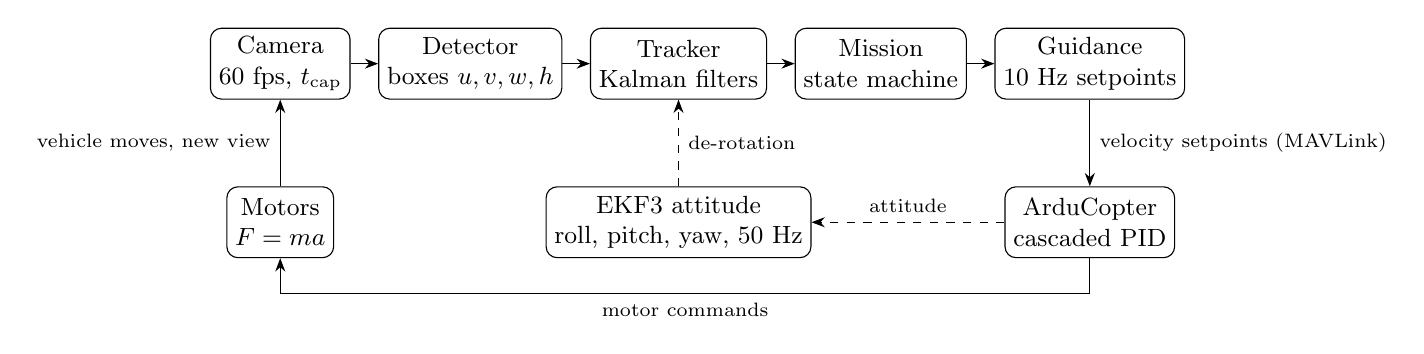
\begin{tikzpicture}[node distance=0.35cm and 0.35cm, box/.style={draw,rounded corners,align=center,font=\small,minimum height=0.9cm,inner sep=3pt}, >=Stealth]
\node[box] (cam) {Camera\\60 fps, $t_\text{cap}$};
\node[box,right=of cam] (det) {Detector\\boxes $u,v,w,h$};
\node[box,right=of det] (trk) {Tracker\\Kalman filters};
\node[box,right=of trk] (mis) {Mission\\state machine};
\node[box,right=of mis] (gui) {Guidance\\10 Hz setpoints};
\node[box,below=1.1cm of gui] (fc) {ArduCopter\\cascaded PID};
\node[box,below=1.1cm of cam] (mot) {Motors\\$F = ma$};
\node[box,below=1.1cm of trk] (ekf) {EKF3 attitude\\roll, pitch, yaw, 50 Hz};
\draw[->] (cam) -- (det); \draw[->] (det) -- (trk); \draw[->] (trk) -- (mis);
\draw[->] (mis) -- (gui); \draw[->] (gui) -- node[right,font=\scriptsize]{velocity setpoints (MAVLink)} (fc);
\draw[->] (fc.south) -- ++(0,-0.45) -| node[pos=0.25,below,font=\scriptsize]{motor commands} (mot.south);
\draw[->] (mot) -- node[left,font=\scriptsize]{vehicle moves, new view} (cam);
\draw[->,dashed] (fc) -- node[above,font=\scriptsize]{attitude} (ekf);
\draw[->,dashed] (ekf) -- node[right,font=\scriptsize]{de-rotation} (trk);
\end{tikzpicture}
\end{center}
\textbf{State estimation} answers ``what is true now, and how sure am I?'' (tracker,
attitude, range, time to contact). \textbf{Control and guidance} answer ``what do I do
about it?'' (pursuit, PN, PID). \textbf{Closed loop}: measure, compare with the goal,
correct, repeat. \textbf{Open loop}: run a fixed plan without looking (today's terminal
segment [G5]).

\section*{1. State and differential equations}
State = the smallest set of numbers that lets you predict the future, given the inputs.
For motion on a line: position $x$ and velocity $v$.
\begin{eqbox}
\[
\frac{dx}{dt} = v,\qquad \frac{dv}{dt} = a
\qquad\Longrightarrow\qquad
\underbrace{\begin{bmatrix} x \\ v\end{bmatrix}_{k+1}}_{\text{next}}
= \underbrace{\begin{bmatrix} 1 & \Delta t\\ 0 & 1\end{bmatrix}}_{F}
\begin{bmatrix} x \\ v\end{bmatrix}_{k}
\quad(\text{constant velocity, } a \approx 0)
\]
\end{eqbox}
A differential equation is a rule for \emph{change}, not a formula for the answer.
The step form is the Euler step: a first-order Taylor approximation, $x(t+\Delta t)\approx
x(t) + x'(t)\Delta t$. \textbf{Matrix times vector}: each output row is a weighted sum of
the inputs. Row 1: new $x = 1\cdot x + \Delta t\cdot v$. Row 2: new $v = v$.
\where{\code{tracker.py}, \code{\_Axis.predict}: \code{self.x += self.r * dt}. Each track
has four such filters: center $u$, center $v$, width $w$, height $h$.}
\begin{exbox}
Box at $u=500$ px, rate 120 px/s, next frame at 60 fps ($\Delta t = 1/60$ s):
predicted $u = 500 + 120/60 = 502$ px.
\end{exbox}

\section*{2. Proportional control and exponential decay}
\begin{eqbox}
\[
v = K_p\, e \;\;\Longrightarrow\;\; \frac{de}{dt} = -K_p\, e
\;\;\Longrightarrow\;\; e(t) = e_0\, e^{-K_p t},\qquad T = \frac{1}{K_p}
\]
\end{eqbox}
\why{you move faster when you are far and slower when you are close, so the error
shrinks by the same \emph{fraction} each second. After $T$: 37\% left. After $3T$: 5\%
left.}
\where{\code{guidance.py}, \code{PurePursuit.command}: $v = K_p q$ with $K_p = 0.8$/s
($T = 1.25$ s). Yaw law \code{yaw\_rate\_command}: $\dot\psi = K_\text{yaw}\,\text{az}$,
$K_\text{yaw} = 1.5$/s. Altitude hold \code{\_altitude\_hold}: $v_D = K_\text{alt}(h -
h_\text{search})$, $K_\text{alt} = 0.5$/s.}

\textbf{Guards on top:} deadband ($|q| \le 0.25$ m $\Rightarrow$ zero), clamp
($|v| \le v_\text{max}$, yaw rate $\le 90^\circ$/s), rate limit
($|v_k - v_{k-1}| \le a_\text{max}\Delta t$, $a_\text{max} = 2$ m/s$^2$).

\textbf{Discrete time:} $e_{k+1} = (1 - K_p\Delta t)\, e_k$. Stable only if
$|1 - K_p\Delta t| < 1$. Too much gain for the step size (or with delay) makes the error
flip sign and grow.
\begin{exbox}
Standoff point 5 m away: command $0.8 \times 5 = 4$ m/s, clamped to $v_\text{max}=3$ m/s.
At 10 Hz the limiter allows $2 \times 0.1 = 0.2$ m/s per step, so 15 steps (1.5 s) to
reach 3 m/s. Yaw: target $30^\circ$ right $= 0.524$ rad $\Rightarrow$ $1.5 \times 0.524
= 0.785$ rad/s $= 45^\circ$/s.
\end{exbox}

\section*{3. Newton, damping, PID, and the cascade}
Thrust is a force, so the vehicle is a \textbf{double integrator}: force $\to$
acceleration $\to$ velocity $\to$ position.
\begin{eqbox}
\[
\ddot x + K_d\,\dot x + K_p\, x = 0,\qquad
\omega_n = \sqrt{K_p},\qquad \zeta = \frac{K_d}{2\sqrt{K_p}},\qquad
\text{overshoot} = e^{-\zeta\pi/\sqrt{1-\zeta^2}}
\]
\[
\text{Try } x = e^{\lambda t}:\quad \lambda^2 + K_d\lambda + K_p = 0
\qquad\text{(the eigenvalues of } A = \begin{bmatrix}0 & 1\\ -K_p & -K_d\end{bmatrix})
\]
\end{eqbox}
\why{$K_p$ is a spring (pulls to the goal), $K_d$ is a damper (resists speed). Real part
of $\lambda$ $<0$: decays. Imaginary part: oscillation. $\zeta<1$ rings, $\zeta=1$ is the
fastest with no overshoot, $\zeta>1$ is sluggish. PID adds $K_i\!\int e\,dt$, which
removes a steady offset (constant wind).}

\textbf{Eigenvector}: a direction the system only stretches or shrinks, never turns. The
eigenvalue is the stretch rate.

\textbf{Cascade (inside ArduCopter, not written by SkyWeave):} position $\to$ velocity
$\to$ acceleration $\to$ lean angles and thrust $\to$ body rates $\to$ motors. Each outer
loop runs several times (about 5--10$\times$) slower than the loop inside it, so it can
treat the inner loop as instant. SkyWeave's 10 Hz velocity setpoints sit on top.

\textbf{Gravity feedforward} (V-D2, planned PN pass): send an \emph{acceleration}
setpoint; ArduCopter adds gravity. Tilt and thrust for a horizontal acceleration $a_h$:
\begin{eqbox}
\[
\theta = \arctan\frac{a_h}{g},\qquad \frac{T}{T_\text{hover}} = \frac{\sqrt{a_h^2 + g^2}}{g}
\]
\end{eqbox}
\begin{exbox}
$K_p = 4$, $K_d = 2$: $\omega_n = 2$, $\zeta = 0.5$, $\lambda = -1 \pm i\sqrt3$, overshoot
$e^{-1.81} \approx 16\%$. Critical damping: $K_d = 4$.
$a_h = 2$ m/s$^2$: tilt $= \arctan(2/9.81) = 11.5^\circ$, thrust $= 1.02\times$ hover.
\end{exbox}

\section*{4. Frames and rotation matrices}
\textbf{NED}: North, East, Down (up is $-z$). \textbf{Body}: $x$ forward, $y$ right, $z$
down. \textbf{Camera}: $X$ image right, $Y$ image down, $Z$ out of the lens.
\begin{eqbox}
\[
R_x(\phi)=\begin{bmatrix}1&0&0\\0&\cos\phi&-\sin\phi\\0&\sin\phi&\cos\phi\end{bmatrix},\;
R_\text{ned,body} = R_z(\psi)\,R_y(\theta)\,R_x(\phi),\;
R^{-1} = R^{\mathsf T},\; \det R = 1
\]
\[
\text{cone\_up: } R_\text{body,cam} = \begin{bmatrix}1&0&0\\0&-1&0\\0&0&-1\end{bmatrix}
\qquad
\hat\ell_\text{ned} = R_\text{ned,body}(t_\text{cap})\; R_\text{body,cam}\; \frac{\text{ray}}{|\text{ray}|}
\]
\end{eqbox}
\why{the \emph{columns} of a rotation matrix are where the source axes land. cone\_up
columns: camera $X$ = body forward, camera $Y$ = body left, camera $Z$ (lens) = body up.
Read the chain right to left: camera $\to$ body $\to$ world. Order matters: rotations do
not commute.}
\where{\code{camera.py}: \code{rot\_x}, \code{rot\_y}, \code{rot\_z}, \code{r\_ned\_body},
\code{MOUNTS}. \code{guidance.py}: \code{derotate}.}

\section*{5. Pinhole camera, de-rotation, timing}
\begin{eqbox}
\[
u = c_x + f\frac{X}{Z},\quad v = c_y + f\frac{Y}{Z}
\qquad\Longleftrightarrow\qquad
\text{ray} = \Big(\frac{u-c_x}{f},\ \frac{v-c_y}{f},\ 1\Big)
\]
\[
f = \frac{960}{\tan 50^\circ} = 805.5 \approx 806 \text{ px (100}^\circ\text{ lens)},\qquad
(c_x, c_y) = (959.5,\ 599.5)
\]
\end{eqbox}
\why{similar triangles. A pixel gives a direction, not a point: depth is lost.}

\textbf{Time alignment [G1]:} use the attitude at the capture time $t_\text{cap}$,
linearly interpolated between the two samples around it, never extrapolated. If the
nearest sample is more than 100 ms away the packet is \emph{attitude-degraded} and
guidance commands zero velocity.
\where{\code{vehicle\_state.py}, \code{VehicleState.attitude\_at}.}

\textbf{World-angle tracking} (V-D10, status: planned, E2a-4): de-rotate each box
center \emph{before} filtering, so the vehicle's own rotation cancels. Today the tracker
filters raw pixels, which slide when the vehicle yaws (probe finding V-S8).

\textbf{Lens distortion} (V-D11, Brown--Conrady): $r_d = r\,(1 + k_1 r^2 + k_2 r^4 + k_3
r^6)$ plus tangential terms $p_1, p_2$. Box centers are undistorted first. Coefficients
are zero until calibration.
\begin{exbox}
403 px off center: $\arctan(403/806) = \arctan 0.5 = 26.6^\circ$. Frame edge:
$\arctan(960/806) = 50.0^\circ$, so a level vehicle sees only targets at least
$90^\circ - 50^\circ = 40^\circ$ above the horizon, within $d_h/\tan 40^\circ = 1.19\,d_h$
horizontally.
Timing: at $45^\circ$/s yaw, a 50 ms stale attitude is $2.25^\circ$ wrong $\approx
806\tan 2.25^\circ \approx 32$ px.
\end{exbox}

\section*{6. Uncertainty and fusing two guesses}
Gaussian: mean (best guess) and variance $\sigma^2$ (spread). About 68\% within
$1\sigma$, 95\% within $2\sigma$.
\begin{eqbox}
\[
K = \frac{\sigma_1^2}{\sigma_1^2 + \sigma_2^2},\qquad
\hat x = x_1 + K\,(x_2 - x_1),\qquad
\sigma^2 = (1-K)\,\sigma_1^2
\quad\Big(\Leftrightarrow\ \tfrac{1}{\sigma^2} = \tfrac{1}{\sigma_1^2} + \tfrac{1}{\sigma_2^2}\Big)
\]
\[
\text{Covariance matrix } P = \begin{bmatrix} p_{00} & p_{01}\\ p_{01} & p_{11}\end{bmatrix}
\;\;(\text{position variance, cross term, velocity variance; draw it as an ellipse})
\]
\end{eqbox}
\why{trust each guess in proportion to its precision ($1/\sigma^2$). The fused estimate
is always tighter than either input.}

\textbf{Two error channels} (project rule): random error goes in the covariance (filter
input); systematic bias (for example a wrong balloon width) is reported, never folded into
the covariance. Averaging does not remove a bias.
\begin{exbox}
$10 \pm 2$ m and $14 \pm 4$ m: $K = 4/20 = 0.2$, $\hat x = 10.8$ m, $\sigma^2 = 3.2$,
$\sigma = 1.79$ m. (Not 12 m: the first guess is 4$\times$ more precise.)
\end{exbox}

\section*{7. The Kalman filter (1D, then 2-state)}
\begin{eqbox}
\[
\textbf{Predict:}\quad \hat x \leftarrow F\hat x,\qquad P \leftarrow F P F^{\mathsf T} + Q
\]
\[
\textbf{Update:}\quad y = z - H\hat x,\quad S = HPH^{\mathsf T} + R,\quad K = P H^{\mathsf T} S^{-1},\quad
\hat x \leftarrow \hat x + K y,\quad P \leftarrow (I - KH)P
\]
\[
F = \begin{bmatrix}1&\Delta t\\0&1\end{bmatrix},\quad H = \begin{bmatrix}1 & 0\end{bmatrix},\quad
Q = \sigma_a^2\begin{bmatrix}\Delta t^4/4 & \Delta t^3/2\\ \Delta t^3/2 & \Delta t^2\end{bmatrix},\quad
R = \sigma_\text{meas}^2
\]
\end{eqbox}
Written out per axis (exactly \code{\_Axis.predict} and \code{\_Axis.update}):
\[
\begin{aligned}
p_{00} &\mathrel{+}= 2\Delta t\,p_{01} + \Delta t^2 p_{11} + q\Delta t^4/4, &
p_{01} &\mathrel{+}= \Delta t\,p_{11} + q\Delta t^3/2, &
p_{11} &\mathrel{+}= q\Delta t^2\\
S &= p_{00} + R, & k_0 &= p_{00}/S,\ \ k_1 = p_{01}/S, & x &\mathrel{+}= k_0 y,\ \ r \mathrel{+}= k_1 y
\end{aligned}
\]
\why{predict: time passes without looking, so uncertainty grows; $F P F^{\mathsf T}$
shears the ellipse (position uncertainty picks up velocity uncertainty times $\Delta t$).
$Q$: the object may accelerate in ways the model does not know (random constant
acceleration per step moves position by $a\Delta t^2/2$ and velocity by $a\Delta t$).
Update: the surprise $y$ corrects the estimate by the gain. We measure only position, but
$k_1 = p_{01}/S$ also corrects velocity, because position and velocity errors are linked.}

\textbf{Gain meaning:} $K\to 1$ trust the sensor; $K \to 0$ trust the model.
\textbf{Tuning:} big $Q$ or small $R$ = responsive but jittery; small $Q$ or big $R$ =
smooth but lags. The ratio matters most.
\where{\code{TrackerConfig}: \code{meas\_sigma\_px} = 2 ($R = 4$ px$^2$),
\code{accel\_sigma\_px\_s2} = 1000 (center axes), \code{size\_rate\_sigma\_px\_s2} = 200
(width, height).}
\begin{exbox}
1D: predicted $u = 510$ px, $P = 12$; measured $520$, $R = 4$. $y = 10$, $S = 16$,
$K = 0.75$, $u = 517.5$ px, $P = 3$ px$^2$.\\
2-state ($\Delta t = 0.1$, $u=500$, $r=100$, $p_{00}=4$, $p_{01}=0$, $p_{11}=400$,
$q = 160000$): predict $u = 510$, $p_{00} = 12$, $p_{01} = 120$; measure 520:
$k_0 = 0.75$, $k_1 = 7.5$/s, $u = 517.5$, $r = 175$ px/s.
\end{exbox}

\section*{8. Many objects: association and the track lifecycle}
\begin{eqbox}
\[
\text{IoU} = \frac{\text{area}(A\cap B)}{\text{area}(A\cup B)},\qquad
d^2_\text{Mahalanobis} = \frac{y^2}{S}\ \ (\text{scalar}),\qquad d^2 = y^{\mathsf T}S^{-1}y\ \ (\text{vector})
\]
\end{eqbox}
\begin{itemize}
\item \textbf{Association} [K2]: greedy pairing by highest IoU between predicted and
detected boxes; never below \code{iou\_min} = 0.1.
\item \textbf{Mahalanobis gate} (planned if needed, E1-D2): the surprise in units of
the expected surprise. $d^2 < 9$ means within $3\sigma$. A coasting track has a large
$S$ and so accepts a wider area.
\item \textbf{M-of-N}: tentative until 3 hits within its first 5 frames (rejects
one-frame false alarms).
\item \textbf{Coasting}: a confirmed track that misses only predicts; $P$ grows. After
more than \code{coast\_cap} = 20 misses (1/3 s at 60 fps) it dies; ids are never reused.
\end{itemize}
\begin{exbox}
Two $100\times100$ boxes, offset 50 px: intersection 5000, union 15000, IoU = 1/3.
\end{exbox}

\section*{9. Nonlinear estimation: EKF and the tangent plane}
\begin{eqbox}
\[
h(x) \approx h(x_0) + J\,(x - x_0),\qquad J_{ij} = \frac{\partial h_i}{\partial x_j}
\qquad(\text{use } J \text{ in place of } F \text{ or } H \text{ in the covariance formulas})
\]
\[
\text{Gnomonic map around a reference } \hat r:\quad
p = \frac{\hat\ell}{\hat\ell\cdot\hat r}\ \ (\text{lies on the plane tangent at } \hat r),\qquad
(\xi, \eta) = (p\cdot e_1,\ p\cdot e_2)
\]
\end{eqbox}
\why{a curved function looks like its tangent plane near a point (Calc 3). The EKF
linearizes around the current estimate every step.}
\begin{itemize}
\item ArduCopter's \textbf{EKF3} fuses gyro (fast, drifts), accelerometer (gravity
direction, noisy), compass, barometer and GPS. Its attitude output feeds de-rotation.
\item \textbf{Why not filter azimuth and elevation} with the camera looking up: the view
is centered on the zenith, where azimuth is singular (like longitude at the North Pole).
The planned tracker filters coordinates on a flat plane touching the unit sphere at the
track's reference direction, and re-centers if the track drifts far (status: planned,
E2a-4).
\end{itemize}

\section*{10. Range from size, and time to contact}
\begin{eqbox}
\[
Z = \frac{f\,W}{w},\qquad r = Z\,|\text{ray}|,\qquad
\frac{dZ}{Z} = -\frac{dw}{w}
\]
\[
\tau = \frac{w}{dw/dt}:\quad w = \frac{fW}{Z}\ \Rightarrow\ \frac{dw}{dt} = -\frac{fW}{Z^2}\frac{dZ}{dt}
\ \Rightarrow\ \frac{w}{dw/dt} = \frac{Z}{-dZ/dt} = \frac{\text{range}}{\text{closing speed}}
\]
\end{eqbox}
\why{similar triangles for range. For $\tau$ the chain rule cancels $f$ and $W$: time to
contact needs no calibration and no balloon size (the ``looming'' cue animals use).}
\where{\code{guidance.size\_range}: valid when $w \ge$ \code{w\_min\_px} = 4 px, else
assume $r = 15$ m clamped to $[1, 60]$ m. $\tau$ (V-D9) is a planned track packet field
(E2a-5); the width filter's rate state already estimates $dw/dt$. Valid only while the box
grows and is not clipped at the frame edge.}
\begin{exbox}
$f = 806$, $W = 1$ m: $w = 403$ px $\Rightarrow Z = 2$ m; $w = 80.6$ px $\Rightarrow
Z = 10$ m. A 2 px width error is 2.5\% (0.25 m) at 10 m but 0.5\% (1 cm) at 2 m. A balloon
of 0.8 m primed as 1 m makes every range 25\% too long (bias).
$w = 403$, $dw/dt = 806$ px/s $\Rightarrow \tau = 0.5$ s; at 2 m that is 4 m/s closing,
and the 0.2 s hand-off happens at 0.8 m.
\end{exbox}

\section*{11. Guidance laws: pure pursuit vs proportional navigation}
\begin{eqbox}
\[
\textbf{Pure pursuit [G3]:}\quad q = p - s\,\frac{p_h}{|p_h|},\quad v = K_p\,q
\qquad\qquad
\textbf{PN (planned):}\quad a_\perp = N\,V_c\,\dot\lambda
\]
\end{eqbox}
\why{\textbf{collision triangle}: if the line of sight (LOS) to the target does not
rotate while the range shrinks, you will collide (sailors: constant bearing, decreasing
range). PN pushes sideways in proportion to how fast the LOS rotates, which drives
$\dot\lambda \to 0$ and leads a moving target. Pure pursuit always points at where the
target is now and ends in a curved tail chase.}

Symbols: $N$ navigation constant (typically 3--5), $V_c$ closing speed (from $\tau$ or
size range), $\dot\lambda$ LOS rotation rate (rad/s) from the world-angle tracker.
\status{PN pass is E2b (V-D2, V-D5, V-D6, V-D12): acceleration setpoints at 50 Hz; steer
until the box touches the frame edge, the track is lost, or $\tau < 0.2$ s; then hold the
last command, brake, climb, \code{pass\_done}. Today: pure pursuit to a standoff point,
then the open-loop terminal segment [G5].}
\begin{exbox}
$N = 3$, $V_c = 4$ m/s, $\dot\lambda = 0.1$ rad/s ($5.7^\circ$/s): $a_\perp = 1.2$
m/s$^2$, a tilt of $\arctan(1.2/9.81) = 7^\circ$.
\end{exbox}

\section*{12. Time, delay, and the mission state machine}
\begin{itemize}
\item \textbf{Rates:} camera 60 Hz, attitude about 50 Hz, guidance 10 Hz (planned 50 Hz in
the pass), ArduCopter inner loops hundreds of Hz.
\item \textbf{Delay is dangerous in feedback}: you correct an error that has already
changed, so you overshoot (the long-pipe shower). Fixes: lower gain, faster loops, predict
forward with the model, time-stamp everything ($t_\text{cap}$), stop steering when the
information gets unreliable ($\tau$ hand-off). ArduCopter also jerk-limits acceleration
input (\code{PSC\_JERK\_NE}, adds lag) and zeroes targets after \code{GUID\_TIMEOUT} = 3 s
with no setpoint.
\item \textbf{Determinism}: mission and guidance never read a clock; time comes from input
stamps, so a recording replays exactly.
\item \textbf{Hybrid system}: discrete states on top of continuous control.
PRIMED $\to$ LAUNCH $\to$ SEARCH (yaw scan $45^\circ$/s, altitude hold) $\to$ ACQUIRING
(confirmed track; yaw toward it) $\to$ ENGAGED (operator approves; pursuit) $\to$ TOUCH
(commit) $\to$ COMPLETE or MISS $\to$ RETURN $\to$ LAND. Side paths: ENGAGED
$\leftrightarrow$ COASTING, LOST $\to$ SEARCH, ABORT $\to$ RETURN, budget and link-loss
failsafes $\to$ RETURN.
\item \textbf{Commit gate [G4]}: $w/1920 \ge \alpha$, $\text{hypot}(u - c_x, v - c_y)
\le \beta\cdot 1920$, track confirmed with $\ge k$ hits, attitude fresh. Estimation
quality gates the control decision.
\end{itemize}

\section*{Symbol table}
\begin{center}
\small
\begin{tabular}{@{}lll@{}}
\toprule
Symbol & Meaning & Typical value (Provisional) \\
\midrule
$u, v, w, h$ & box center and size in pixels & 1920 $\times$ 1200 grid \\
$f,\ c_x,\ c_y$ & focal length, image center (px) & 806, 959.5, 599.5 \\
$t_\text{cap}$ & frame capture time (board ms) & 60 fps \\
$K_p,\ K_\text{yaw},\ K_\text{alt}$ & proportional gains & 0.8, 1.5, 0.5 per s \\
$v_\text{max},\ a_\text{max}$ & speed cap, command rate limit & trial value, 2 m/s$^2$ \\
$P,\ Q,\ R$ & state, process, measurement covariance & $R = 4$ px$^2$ \\
$K$ & Kalman gain & between 0 and 1 \\
$y,\ S$ & innovation (surprise), its variance & \\
$W,\ Z,\ r$ & target width, depth, range & $W = 1$ m \\
$\tau$ & time to contact & hand-off at 0.2 s \\
$N,\ V_c,\ \dot\lambda$ & PN constant, closing speed, LOS rate & 3--5 \\
$\zeta,\ \omega_n$ & damping ratio, natural frequency & \\
\code{coast\_cap}, M-of-N & misses before death, confirmation & 20, 3 of 5 \\
\bottomrule
\end{tabular}
\end{center}

\end{document}
